%-------------------- Packages --------------------%

\documentclass[11pt,a4paper]{report}
\usepackage[utf8]{inputenc}
\usepackage[french]{babel}
\usepackage[T1]{fontenc}
\usepackage{amsmath} %pour les formules maths
\usepackage{amsfonts}
\usepackage{amssymb}
\usepackage{graphicx} %pour inclure des images
\usepackage{hyperref} %pour les lien URLs
\usepackage[left=2cm,right=2cm,top=3cm,bottom=3cm]{geometry}
\usepackage{pifont} %pour les puces spéciales
\usepackage{listings} %pour écrire du code
\usepackage{xcolor} %pour la mise en couleur
\usepackage{multirow} %pour les tableaux
\usepackage{bclogo} %pour des boîtes texte avec un logo


%-------------------- New Colors --------------------%

%Basic

\definecolor{purple}{rgb}{0.6, 0.2, 0.9}

%Dark
\definecolor{dkgreen}{rgb}{0,.6,0}
\definecolor{dkblue}{rgb}{0,0,.6}
\definecolor{dkyellow}{cmyk}{0,0,.8,.3}
\definecolor{dkred}{rgb}{0.6, 0, 0}


%Light
\definecolor{ltblue}{rgb}{0.67, 0.85, 0.9}
\definecolor{ltred}{rgb}{0.8, 0.32, 0.32}
\definecolor{ltgrey}{rgb}{0.94,0.94,0.94}



%-------------------- Config lstlisting --------------------%

\lstset{
language=php,
basicstyle=\ttfamily\tiny, %
identifierstyle=\color{dkred}, %
keywordstyle=\color{dkblue}, %
stringstyle=\color{dkgreen}, %
commentstyle=\it\color{gray}, %
emph=[1]{php},
emphstyle=[1]\color{black},
emph=[2]{if,and,or,else},
emphstyle=[2]\color{dkyellow},
emph=[3]{imap_open, imap_close, imap_fetch_overview, imap_check, imap_list, imap_mail_move, imap_search, imap_fetchstructure			},
emphstyle=[3]\color{dkblue},
emph=[4]{string, int, double, float, private, public, static, bool, resource, array, object},
emphstyle=[4]\color{purple},
columns=flexible, %
tabsize=2, %
extendedchars=true, %
showspaces=false, %
showstringspaces=false, %
numbers=left, %
numberstyle=\tiny, %
breaklines=true, %
breakautoindent=true, %
captionpos=b, %
backgroundcolor=\color{ltgrey}
}

%-------------------------------------%
\newcommand{\quest}[2]{\textcolor{dkblue}{\textit{#1}}\vspace*{.2cm}\par\hspace*{.5cm}#2}

\newcommand{\vrai}[0]{\textcolor{dkgreen}{Vrai}}
\newcommand{\faux}[0]{\textcolor{dkred}{Faux}}

\author{Wéry Benoît}
\title{Préparation à l'examen de \textit{Systèmes d'exploitation}}
\date{\today}


\begin{document}
\maketitle

%---------------------%
\chapter{Définitions de concepts}
%---------------------%

\begin{enumerate}\setlength\itemsep{1em}
%--- 1 -------------------------------%
\item\quest{Définissez ce qu’est le système d’exploitation d’un système informatique. En particulier, identifiez ses buts et les abstractions du système informatique qu’il permet d’opérer. Présentez également
la structure d’un système informatique et où il s’y situe.}
{
Le système d'exploitation (Operating System = OS) est une \textbf{couche logicielle intermédiaire} entre l'utilisateur et le hardware.
\begin{figure}[h!]
\center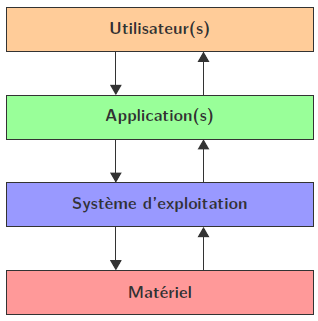
\includegraphics[scale=.4]{images/couches-si}
\caption{Vue en couches du système informatique \cite{ref1}}
\end{figure}
\paragraph{}
Ses principaux objectifs sont:
\begin{enumerate}
\item \textbf{Pratique}: permettre une utilisation facile du système informatique (SI) pour l'utilisateur
\item \textbf{Efficace}: optimiser l'utilisation du hardware
\item \textbf{Evolution}: ajouter de nouvelles fonctions systèmes
\end{enumerate}

Parmi les \textit{abstractions} que l'OS propose, on retrouve les suivantes:
\begin{figure}[h!]
\center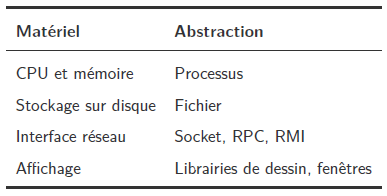
\includegraphics[scale=.5]{images/abstractions-OS}
\caption{Abstractions proposées par l'OS \cite{ref1}}
\end{figure}

\paragraph{}
L'OS fournit un environnement pour utiliser les ressources (matériel, logiciel et données) du système informatique.

\paragraph{Exemples d'OS: } Windows10, macOS, Android, Ubuntu, Debian, Solaris,...

\paragraph{Remarques:}
\begin{enumerate}
\item L'OS facilite l'exploitation du hardware MAIS il n'est pas indispensable au fonctionnement du SI.
\end{enumerate}
}


%--- 2 -------------------------------%
\item\quest{Quelles sont les principales étapes qui sont franchies lors du démarrage d’un système informatique ? Citez-les et identifiez la fonction de chacune des étapes, c’est-à-dire le rôle des actions réalisées pour le fonctionnement du système informatique.}
{
\begin{enumerate}
\item Le "programme initial" (boostrap), stocké dans la ROM, initialise plusieurs aspects du système: registres CPU, contrôleur périphérique, contenu de la mémoire,...
\item Ensuite, il localise et charge dans la RAM le noyau de l'OS (càd le kernel)
\item Le kernel exécute des processus systèmes (démons), tel que "init", qui eux-même en lancent d'autres,...
\item Lorsque tous les démons ont été lancés, le démarrage est complété et l'OS se met en attente d'un évènement
\end{enumerate}
}


%--- 3 -------------------------------%
\item\quest{Citez et expliquez des exemples de services offerts par un système d’exploitation. Comment
peut-on les classer selon le type destinataire du service ? Citez et expliquez également les trois
aspects sur lesquels il joue le rôle de coordinateur.}
{
L'OS peut être vu comme un \textit{fournisseurs de services} pour l'utilisateur et les programmes. Parmi ces services, on retrouve:
\begin{enumerate}
\item L'\textcolor{ltred}{\textsc{exécution de programmes}}: l'OS charge en mémoire et exécute un programme
\item Les \textcolor{ltred}{\textsc{opérations d'Entrée/Sortie}}: gestion des périphériques, interactions utilisateur
\item La \textcolor{ltred}{\textsc{manipulation du système fichiers}}: il gère la lecture et l'écriture des fichiers, les permissions d'accès, les propriétaires,...
\item La \textcolor{ltred}{\textsc{communication entre processus}}: l'OS définit quel processus a accès à quelle partie de mémoire,...
\item La \textcolor{ltred}{\textsc{détection d'erreur}}: répère les erreurs au niveau du CPU, de la mémoire, des périph, du réseau,... et tente des les corriger
\item L'\textcolor{ltred}{\textsc{allocation des ressources}}: distribution des ressources (CPU, mémoire,...) entre les différents processus exécutés
\item La \textcolor{ltred}{\textsc{comptabilisation}}
\item La \textcolor{ltred}{\textsc{protection}} et la \textcolor{ltred}{\textsc{sécurité}}: authentification utilisateurs,...
\end{enumerate}

\paragraph{}
Ces services peuvent être regroupés en deux catégories selon le destinataire:
\begin{enumerate}
\item Services pour l'\textsc{utilisateur}
\item Services pour le \textsc{système}
\end{enumerate}

\begin{figure}[h!]
\center
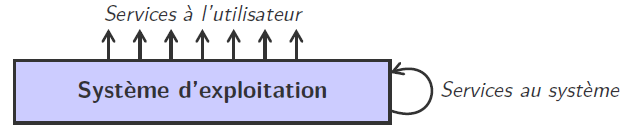
\includegraphics[scale=.5]{images/types-services}
\caption{Catégories de services de l'OS}
\end{figure}

\paragraph{}
L'OS joue également un rôle de \textbf{coordinateur} sur trois aspects:
\begin{enumerate}
\item \textcolor{ltred}{\textsc{Protection}}: il s'assure que les jobs n'interfèrent pas les uns avec les autres
\item \textcolor{ltred}{\textsc{Communication}}: il doit permettre aux jobs de pouvoir intéragir entre eux
\item \textcolor{ltred}{\textsc{Gestion des ressources}}: il facilite le partage des ressources (CPU,mémoire,...) entre les jobs
\end{enumerate}
}


%--- 4 -------------------------------%
\item\quest{Qu’est-ce-que la multiprogrammation ? Quelles conséquences cette tendance a-t-elle eue sur le
développement des systèmes d’exploitation ?}
{
\begin{figure}[h!]
\center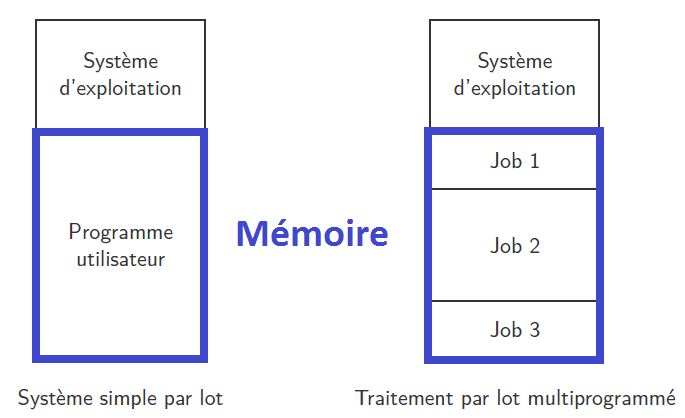
\includegraphics[scale=.4]{images/multiprogrammation}
\caption{Répartition des programmes en multiprogrammation \cite{ref1}}
\end{figure}

Dans le cas de la multiprogrammation, plusieurs jobs sont mis en mémoire simultanément. Chaque job possède \textbf{son propre espace mémoire} qui n'est pas accessible par les autres (Rem: dans certains cas, plusieurs jobs peuvent partager une même zone mémoire, si cela est demandé).
\paragraph{}
Contrairement au système simple, si un job est en attente d'une réponse, alors l'OS peut choisir d'en lancer un autre. Ainsi, on donne l'\textit{illusion} de faire tourner plusieurs jobs en même temps. On parle de \textbf{concurrence}, car le CPU est \textit{multiplexé} entre plusieurs tâches qui sont exécutées les unes après les autres et non pas en même temps (parallélisme).

\paragraph{}
Cette approche a eu pour conséquence la nécessité de gérer les éléments suivants:
\begin{enumerate}
\item l'\textbf{attribution des ressources}
\item la \textbf{gestion de la mémoire} allouée aux tâches
\item la \textbf{planification} de l'utilisation du CPU, càd des tâches à exécuter
\end{enumerate}

\paragraph{A vérifier...}
Il y a un partage des \textit{ressources} et du \textit{temps-calcul} qui se fait à deux niveaux:
\begin{enumerate}
\item D'une part, \textit{plusieurs batch de jobs} via la multiprogrammation
\item D'autre part, \textit{plusieurs utilisateurs} avec le time-sharing
\end{enumerate}
}


%--- 5 -------------------------------%
\item\quest{Citez et expliquez les deux modes d’exécution possible d’un programme. Qu’est-ce-qu’un appel
système et comment se déroule l’exécution d’un tel appel ?}
{
Un programme peut être utilisé dans deux modes d'exécution:
\begin{enumerate}
\item mode \textcolor{ltred}{\textsc{noyau}}: code destiné à l'OS (ces instructions ont plus de privilèges). Dans ce mode, l'OS a un accès complet à l'ensemble du matériel et peut exécuter n'importe qu'elle instruction (que la machine est capable de traiter)
\item mode \textcolor{ltred}{\textsc{utilisateur}}: code destiné à l'utilisateur (ex: les programmes/softwares). Dans ce mode, les logiciels n'ont accès qu'à une partie des instructions possibles.
\end{enumerate}
%\begin{figure}[h!]
%\center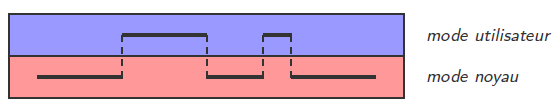
\includegraphics[scale=.5]{images/modes-utilisation-programme}
%\caption{Modes d'exécutions d'une instruction \cite{ref1}}
%\end{figure}


\paragraph{}
Un \textbf{appel système} permet d'utiliser un service de l'OS, il s'agit d'une tâche très \textit{bas niveau}. Les appels systèmes disponibles dépendent de l'OS et sont utilisés par des \textbf{programmes systèmes}.

\paragraph{}
Afin de ne pas ré-écrire soi-même les séquences des nombreux appels systèmes d'un service, on utilise une \textbf{API} (Application Programming Interface -> !! interface au sens de "contrat", classe purement abstraite) via une \textit{librairie}
\paragraph{}
Lors de l'exécution d'un appel système, le programme passe du mode utilisateur au mode noyau. Le passage d'un mode à l'autre est géré par l'\textit{interface des appels systèmes} qui intercepte ces appels sys. dans l'API.
\paragraph{}
Ainsi, le programme utilisateur n'a pas connaissance du détails des différents appels sys. Il respecte simplement l'utilisation de l'API (noms fonctions, passage des bons paramètres,...) et comprend la valeur de retour.
\begin{figure}[h!]
\center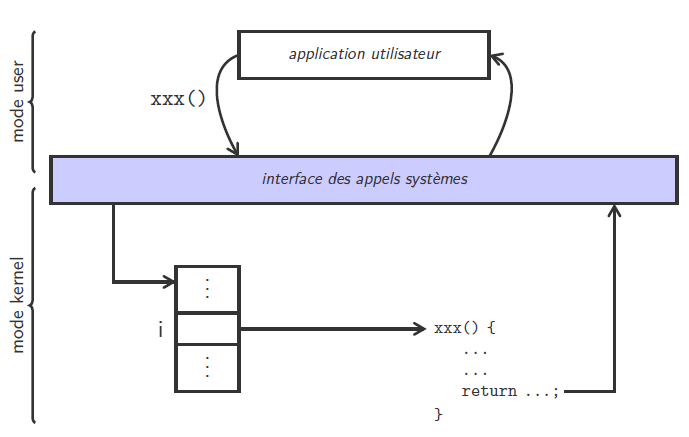
\includegraphics[scale=.5]{images/execution-appel-systeme}
\caption{Changement de mode via l'\textit{interface des appels systèmes} \cite{ref1}}
\end{figure}
}


%--- 6 -------------------------------%
\item\quest{Définissez le concept de processus et détaillez les différentes opérations que l’on peut réaliser depuis sa création jusque sa terminaison. Citez et expliquez quels sont les différents états possibles d’un processus.}
{
Un processus est un \textbf{programme en cours d'exécution}. Pour rappel, un programme peut se retrouver dans deux états:
\begin{enumerate}
\item Passif : stocké sur le disque dur et inactif
\item Actif: lancé par l'OS, il est alors placé en mémoire RAM (on parle ici de processus)
\end{enumerate}
\paragraph{}
Plusieurs processus peuvent être associés à un même programme. Ex: L'OS, qui est un programme, possède un processus nommé le "dispatcher".


\paragraph{}
Un processus est une \textbf{abstraction} qui représente une activité, il est représenté par un \textbf{bloc mémoire structuré} dans la RAM.
L'OS attribue à chaque processus une zone mémoire, qui lui est réservée, dans laquelle sont stockées les informations suivantes:
\begin{enumerate}
\item zone texte: code du programme
\item pile: données temporaires
\item tas: mémoire dynamiquement allouée
\item zone de données: variables globales
\end{enumerate}

\paragraph{}
Un processus peut être créé à différents moments:
\begin{enumerate}
\item Initialisation du système
\item Aooel système
\item Requête utilisateur
\item Initialisation d'un travail en traitement par lots
\end{enumerate}

\paragraph{OPERATIONS...}

\paragraph{Les différents états...}
Dans les versions les plus complètes, on distingu jusqu'à 7 états différents que peut prendre un processus.
\begin{itemize}
\item NEW: en cours de création
\item RUNNING: instructions en cours d'exécution
\item WAITING: en attente d'un évènement
\item READY: prêt et en attente du CPU
\item TERMINATED: exécution terminée
\item WAITING/SUSPENDED: swappé sur le disque dur et en attente d'un évènement
\item READY/SUSPENDED: swappé sur le disque dur et prêt à être exécuté
\end{itemize}

\paragraph{}
Lorsqu'un nouveau processus est créé, il est placé dans la file des processus READY, en attendant d'être choisi par l'OS pour son exécution. Lorsque son temps imparti est terminé, soit le processus a pu être fini, dans quel cas il est passé à l'état TERMINATED, soit il n'est pas fini et est alors replacé dans la file d'attente READY.
\paragraph{}
Si un processus doit obtenir une valeur, un évènement, ... il est retiré du CPU et placé en état WAITING, dans une nouvelle file, jusqu'à ce qu'il obtienne sa réponse. Après cela, il pourra alors retourné dans l'état READY.
\paragraph{}
Lorsqu'il n'y a plus assez de place en mémoire RAM, l'OS peut décider de déplacer certains processus vers la mémoire du disque dur. Cette transistion s'appelle le \textit{swapping} et amène le proc. dans un état SUSPENDED. AU moment de son activation, il sera remplacé dans la RAM.
}


%--- 7 -------------------------------%
\item\quest{Comment et où le système d’exploitation maintient-il de l’information par rapport aux processus? Quel genre d’informations garde-t-il et pourquoi ?}
{
L'OS maintient en mémoire une table des processus qui contient un \textbf{bloc de contrôle} pour chaque processus.
Ces blocs stockent des informations spécifiques telles que:
\begin{itemize}
\item l'état du processus, son identification (PID) et un compteur ordinal (retient la position courante du processus à la fin de sa dernière exécution)
\item les valeurs des registres du CPU (pour sauvegarde)
\item la zone allouée dans la RAM (les adresses limites)
\item une liste des fichiers ouverts par le processus
\item ...
\end{itemize}

Lorsqu'un processus est terminé, l'OS met à jour le bloc de contôle qui lui est associé. Lorsqu'il doit charger le processus pour exécution, il utilise les données courantes du bloc.
}


%--- 8 -------------------------------%
\item\quest{Quelles sont les différences entre parallélisme et concurrence ? Comment les obtient-on dans un système informatique donné ? Le hardware disponible est-il un facteur déterminant dans le choix
entre parallélisme et concurrence lors du développement d’un programme ?}
{
\paragraph{Parallélisme...} plusieurs tâches sont effectuées simultanément sur les coeurs différents
\paragraph{Concurrence...} le CPU \textit{donne l'illusion} de faire tourner plusieurs tâches en leur attribuant les ressources tour-à-tour

\paragraph{}
Pour pratiquer du parallélisme, il faut nécessairement avoir un CPU multicoeurs ou plusieurs CPU physiques!!

\paragraph{Remarque...} On distingue deux niveaux de parallélisme: para. \textit{de données} (répartition sur plusieurs coeurs des données à traîter par une même tache) et para. \textit{de tâches} (exécution de différentes tâches sur plusieurs coeurs).
}


%--- 9 -------------------------------%
\item\quest{Citez et caractérisez les deux types de threads en fonction du niveau où le support des threads est fourni. Citez, expliquez et comparez les différents mappings que l’on peut réaliser entre ces
deux types de thread.}
{
/!\ /!\ à compléter
\paragraph{}
Un thread est "découpage" d'un processus  (c'est en quelque sorte "un processus dans un processus"), une unité d'exécution liée au processus et qui chargée d'en exécuter une partie. Plusieurs threads issus d'un même processus partagent certaines ressources (le code, les données et les fichiers ouverts) et possèdent des informations qui leurs sont propres (un identifiant, des registres et un pile). IMAGE...

\paragraph{}
On distingue les threads au niveau \textbf{utilisateur} et \textbf{noyau}.


\paragraph{1) Threads utilisateurs}
Le noyau gère les processus et  ne se préoccupe pas de l'existence des threads. Donc, lorsqu'il alloue le processeur à un processus, le temps est réparti entre les différents threads et cet ordonnancement est la responsabilité de l'application elle-même (utilisation de foncions telles que: slepp(), suspend(), reusme(), stop()... présentent dans des librairies spécifiques).
\paragraph{}
Ce système est donc totalement indépendant de l'OS sur lequel il tourne. Par contre, il ne peut pas être utilisé en multiprocesseurs et un appel système d'un thread peut bloquer tout le processus.
IMAGES DOCUMENT ANNEXE

\paragraph{2) Theads noyau}
L'OS gère lui-même l'ordonnancement des threads, au même titre que les processus, en leur allouant du temps CPU. Dans ce cas ci, si un thead est bloqué, ce n'est pas tout le processus qui est bloqué puisque d'autres threads (de ce même processus) peuvent être exécutés. Contrairement au threads utilisateurs, les threads d'un processus peuvent être répartis sur différents coeurs (multi-threading) MAIS, le changement de contexte nécessite de passer par le noyau...
}


%--- 10 -------------------------------%
\item\quest{Définissez ce qu’est et ce que fait l’ordonnanceur de processus, et le dispatcher. Quand ces derniers sont-il exécutés ? Qu’est-ce-que la préemption et quels sont ses avantages et inconvénients ?}
{
L'\textbf{ordonnanceur court terme} est un processus OS qui \textbf{choisit} le processus de la \textit{ready queue} qui sera envoyé sur le CPU. Il alterne donc les processus qui sont maintenus en mémoire pour qu'il ait acces aux ressources chacun à leur tour.
\paragraph{}
On distingue 4 instants où l'ordonnanceur doit prendre une décision:
\begin{enumerate}
\item Lorsqu'un p. passe de l'état Running à Waiting
\item Lorsqu'un p. passe de l'état Running à Ready
\item Lorsqu'un p. passe de l'état Waiting à Ready
\item Lorsqu'un p. se termine
\end{enumerate}

\paragraph{}
Le \textbf{dispatcher} est un processus OS qui \textbf{donne} le contrôle du CPU à un processus. Il doit...
\begin{enumerate}
\item Initialiser tout ce qu'il faut pour lancer le p. (celui choisi par l'ordonnanceur). Pour cela, il regarde dans la \textit{table des processus} le \textit{bloc de contrôle} de ce processus.
\item Il bascule en mode utilisateur (changement de 1 bit)
\item Il se positionne à la bonne adresse mémoire pour relancer le p.
\end{enumerate}

\paragraph{}Chaque dispatch engendre un \textbf{temps de latence} (temps "perdu" pour l"utilisateur), il est donc important que ce dispatcher soit le plus rapide possible.

\paragraph{Rappel préemption...} un système/OS est dit préemptif s'il peut interompre à tout instant une tâche en cours d'exécution. On distingue ainsi les ordonnanceurs préemptifs (un processus garde le contrôle CPU jusqu'à ce qu'il le relâche) des ordonnanceurs non-préemptifs (un p. peut être retiré à tout moment du CPU -> ex: interruption, niveaux de priorités,...)
\paragraph{}
Dans le dernier cas, si un processus peut être interrompu avant son arrêt "normal" (tâche terminée, changement état volontaire), il faut mettre un place des mécanismes, par exemple: dans le cas de données partagées, il faut montrer que la donnée utilisée n'est plus à jour,...

\paragraph{/! /! /!}
Dans un cas préemptif, dès qu'un processus arrive, l'OS doit reprendre la main pour calculer la priorité de ce p. et prendre une décision (algo. ordonnancement). Ces "pauses" diminuent le temps en mode "utilisateur", il faut donc que le travail soit fait le plus vite possible.

\paragraph{}
Plusieurs critères existent afin d'évaluer la qualité d'un ordonnanceur:
\begin{enumerate}
\item l'\textsc{Utilisation CPU}: le pourcentage de temps où le CPU est occupé
\item le \textsc{débit} de processus: nombre de processus terminés par unité de temps
\item le \textsc{temps de rotation}: temps total écoulé pour l'exécution d'un processus
\item le \textsc{temps d'attente}: somme des temps d'attente en ready queue
\item \textsc{temps de réponse}: temps entre la soumission du p. et sa première réponse
\end{enumerate}

\paragraph{}
En fonction, du contexte on cherchera à optimiser certains critères soit par rapport à une valeur moyenne soit par rapport aux valeurs extremes (max et min).

\paragraph{Exemples d'algorithmes d'ordonnancement...}
\textit{First-Come First-Served} (FCFS), \textit{Shortest-Job-First} (SJF), \textit{Shortest-Reaming-Time-First}, \textit{Round-Robin} (RR)... Il est possible de mettre en place un système de "files de processus" (en fonciton du type de p.) qui ont chacunes leur propre algo.
}

%--- 11 -------------------------------%
\item\quest{Définissez ce qu’est une section critique et dans quelle situation l’existence d’une telle section peut poser problème (illustrez avec un exemple). Citez et expliquez une solution que l’on peut
apporter pour protéger de telles sections en synchronisant des processsus.}
{}


%--- 12 -------------------------------%
\item\quest{Définissez ce qu’est un deadlock et dans quelles situations il peut se produire (illustrez avec un exemple). Comment peut-on détecter, prévenir et se remettre d’un deadlock ?}
{}


%--- 13 -------------------------------%
\item\quest{Citez et expliquez les différents moyens que l’on peut mettre en oeuvre pour faire communiquer
entre eux des processus coopératifs ? Quels sont les avantages et inconvénients de ces deux
moyens de communication ?}
{}


%--- 14 -------------------------------%
\item\quest{Expliquez ce qu’est le principe d’adressage ? Comment l’unité mémoire intervient-elle ? Définissez et expliquez le principe de liaison des adresses.}
{}


%--- 15 -------------------------------%
\item\quest{En quoi consiste le swapping ? Citez et expliquez les différentes formes de swapping qu’il existe, et comparez-les.}
{}


%--- 16 -------------------------------%
\item\quest{Citez, expliquez et comparez les différentes stratégies d’allocation de la mémoire que l’on peut mettre en place. Quels sont les risques de fragmentation liés à ces stratégies ?}
{}


%--- 17 -------------------------------%
\item\quest{Expliquez le principe de la segmentation. En quoi est-il plus proche de la pensée du programmeur? Comment les adresses sont-elles construites lorsqu’on utilise la segmentation ?}
{}


%--- 18 -------------------------------%
\item\quest{Expliquez le principe de la pagination. Quels sont ses avantages par rapport à la segmentation? Comment les adresses sont-elles construites lorsqu’on utilise la pagination ? Comment peut-on améliorer les performances de la pagination à l’aide d’une mémoire spécialisée ?}
{}


%--- 19 -------------------------------%
\item\quest{Citez et expliquez les différentes structures que l’on peut utiliser pour stocker la table des pages.
Quels sont les avantages et inconvénients de ces structures ? Dans quelles situations sont-elles
plus adaptées ?}
{}


%--- 20 -------------------------------%
\item\quest{Définissez et expliquez les différences et les liens entre mémoire physique et mémoire virtuelle. Comment le système d’exploitation fait-il le lien entre ces deux mémoires, pour les différents processus ?}
{}
%--- 21 -------------------------------%
\item\quest{Définissez et expliquez le concept de défaut de page. Quand un défaut de page se produit-il ? En quoi altèrent-ils les performances du système ?}
{}


%--- 22 -------------------------------%
\item\quest{Définissez, expliquez et comparez les différentes stratégies que l’on peut mettre en place pour allouer les cadres.}
{}


%--- 23 -------------------------------%
\item\quest{Définissez la notion d’écroulement et expliquez en quoi elle rend un système instable. Comment
peut-on détecter et se protéger d’un écroulement ?}
{}


%--- 24 -------------------------------%
\item\quest{Définissez la notion de fichier et expliquez comment le système d’exploitation les gère. Citez et expliquez des exemples d’opérations qu’il est possible de réaliser sur des fichiers.}
{}


%--- 25 -------------------------------%
\item\quest{Expliquez comment un disque peut être structuré en partition/volume/systèmes de fichiers.
Citez, expliquez et comparez différentes manières de concevoir une structure en répertoires.}
{}


%--- 26 -------------------------------%
\item\quest{Définissez ce qu’est un système de fichiers et les informations que le système d’exploitation
retient pour l’organiser. En quoi consiste le montage d’un système de fichiers et qu’est-ce-que le
système de fichiers virtuel ?}
{}


%--- 27 -------------------------------%
\item\quest{Citez, expliquez et comparez les différentes méthodes d’allocation utilisées pour stocker les
fichiers sur le disque.}
{}


%--- 28 -------------------------------%
\item\quest{Citez et expliquez les deux types de formatage d’un disque qu’il est possible de réaliser. Quels sont les buts précis de chacun de ces deux formatages ?}
{}


%--- 29 -------------------------------%
\item\quest{Citez, expliquez et comparez les différentes structures RAID qu’il est possible de mettre en
oeuvre. Dans quel cas concret utiliseriez-vous l’une ou l’autre structure ?}
{}


%--- 30 -------------------------------%
\item\quest{Définissez ce qu’est un driver de périphérique. Où ce dernier intervient-il et avec quels autres composants interagit-il afin de permettre à un utilisateur d’exploiter un périphérique.}
{}

%--- 31 -------------------------------%
\item\quest{Citez et expliquez la notion de machine virtuelle et quelles sont les deux types de machines
virtuelles qu’il est possible de mettre en oeuvre.}
{}


%--- 32 -------------------------------%
\item\quest{Quelles sont les différences entre moniteur de machines virtuelles et système d’exploitation ?
En particulier, quelles sont les opérations qu’ils doivent tous les deux faire et celles qui les
distinguent.}
{}


%--- 33 -------------------------------%
\item\quest{Quelles sont les similitudes et différences entre les deux types d’hyperviseur. Quels sont les
avantages et inconvénients de ces deux types d’hyperviseur ?}
{}


%--- 34 -------------------------------%
\item\quest{Quelles sont les différences entre le kernel Linux, un système Linux et une distribution Linux. Mettez votre comparaison en parallèle avec les trois composants principaux de Linux qui sont en
accord avec Unix.}
{}


%--- 35 -------------------------------%
\item\quest{Définissez et expliquez ce que sont les modules kernel. En particulier, expliquez à quoi ils servent, en quoi ils permettent d’obtenir un kernel minimal et en quoi ils facilitent le développement de
drivers.}
{}


%--- 36 -------------------------------%
\item\quest{La création d’un nouveau processus en Linux passe par deux appels systèmes. Citez-les et
expliquez leur rôle. Quels avantages apporte un tel choix de design en comparaison à Windows où
un nouveau processus est directement créé avec un unique appel à l’appel système CreateProcess.}
{}

%--- 37 -------------------------------%
\item\quest{Expliquez le modèle CIA+ en détaillant chacun des objectifs visés.}
{}


%--- 38 -------------------------------%
\item\quest{Donnez et expliquez trois principes de conception pour le développement de mécanismes de
protection.}
{}


%--- 39 -------------------------------%
\item\quest{Expliquez comment construire un certificat de clé publique, et comment on peut vérifier l’authenticité
de la clé.}
{}

%--- 40 -------------------------------%
\item\quest{Expliquez ce qu’apporte l’utilisation du « sel »dans le stockage de mots de passe.}
{}
%--- 41 -------------------------------%
\item\quest{Expliquez le contrôle d’accès aux fichiers Unix classique, ainsi que son extension en « Access
List ».}
{}

\end{enumerate}


\chapter{Raisonnement}
\begin{enumerate}\setlength\itemsep{1em}
%--- 1 -------------------------------%
\item\quest{Citez, expliquez et comparez différentes approches possibles pour structurer le code d’un système d’exploitation. Quels sont les avantages et inconvénients de ces différentes approches en fonction
du système informatique à opérer ? Argumentez.}
{}

%--- 2 -------------------------------%
\item\quest{Définissez ce que sont les threads et comparez-les par rapport aux processus. Que permettent-ils de plus, par rapport à un système d’exploitation ne proposant que des processus ? Confondre
les threads et les processus en un seul type d’entité comme le fait Linux est-il intéressant ?
Argumentez.}
{}


%--- 3 -------------------------------%
\item\quest{Citez, expliquez et comparez différentes stratégies d’ordonnancement que l’on peut mettre en oeuvre (FCFS, SJF, priorité, RR, files multi-niveaux). Comment peut-on les comparer ? Y a-t-il
un meilleur algorithme dans l’absolu ? Argumentez.}
{}


%--- 4 -------------------------------%
\item\quest{L’acquisition de ressources par des processus peut conduire le système dans des états de deadlock. Il existe plusieurs stratégies permettant d’éviter ou de se remettre d’un deadlock. Quelles
sont-elles et en quoi elles sont plus ou moins adaptées selon le type de système informatique ?
Argumentez.}
{}


%--- 5 -------------------------------%
\item\quest{L’utilisation de threads en lieu et place de processus facilite-t-il la communication entre ces entités ? Est-on limités aux mêmes mécanismes de communication ? Où y gagne-t-on et que
perd-on ? Argumentez.}
{}


%--- 6 -------------------------------%
\item\quest{Citez, expliquez et comparez différentes stratégies de remplacement des pages que l’on peut
mettre en oeuvre (FIFO, optimal, LRU, approximation de LRU, LFU, MFU). Comment peut-on
les comparer ? Y a-t-il un meilleur algorithme dans l’absolu ? Argumentez.}
{}


%--- 7 -------------------------------%
\item\quest{Un système d’exploitation peut adopter plusieurs attitudes différentes suite à l’apparition
d’un deadlock. Citez-les et expliquez en quoi elles sont plus adaptées en fonction du système
d’exploitation à opérer. Argumentez.}
{}


%--- 8 -------------------------------%
\item\quest{Citez, expliquez et comparez différentes stratégies d’ordonnancement de disque l’on peut mettre en oeuvre (FCFS, SSTF, SCAN, C-SCAN, LOOK, C-LOOK). Comment peut-on les comparer ?
Y a-t-il un meilleur algorithme dans l’absolu ? Argumentez.}
{}


%--- 9 -------------------------------%
\item\quest{Une virtualisation est réussie si le système d’exploitation est incapable de savoir s’il tourne sur une machine physique ou sur une virtuelle. Expliquez comment un système d’exploitation
pourrait se rendre compte qu’il est trompé et ce qu’on peut mettre en oeuvre pour le tromper.}
{}


%--- 10 -------------------------------%
\item\quest{Dans plusieurs situations (ordonnancement de processus, remplacement de pages, ordonnancement
d’opérations disque), plusieurs algorithmes sont possibles. Y a-t-il à chaque fois un algorithme
qui est le meilleur dans tous les cas ? Comment peut-on comparer ces algorithmes ? Sont-ils
bon ou mauvais selon le système informatique à opérer ? Comment choisir du mieux possible
l’algorithme à utiliser étant donné un système d’exploitation ? Argumentez.}
{}

%--- 11 -------------------------------%
\item\quest{Vous devez installer un serveur web sécurisé, sur base d’un OS Linux. Comment procédez-vous ?
Détaillez les grandes lignes de votre stratégie de hardening.}
{}
\end{enumerate}

\end{document}
